\section{Applications for Large Models}

In this section, we look at three modeling applications. The first one is software modeling, which is what most of the MODELS community is concerned with and what the modeling frameworks mentioned in this paper were designed for. But techniques originally developed for software modeling are also used for other applications. More abstractly, software modeling can be explained as the representation, analysis, and manipulation of structured data. 

Our research group, for example, uses EMF to represent and analyse sensor data received from our wireless sensor network test-bed (\emph{Humboldt Wireless Lab}~\cite{hwl}). Models of heterogeneous sensor data will be our second application. 
This application is what actually motivated us as authors for this work, because existing approaches where either impractical (lazy loading of EMF resources), or far to slow to store the data at the rate it was produced (CDO and manual relational data base persistence). 
Refer to our publications~\cite{1,2} for more details. 

The third application that we want to analyse, are geo-spatial models and more specifically 3D object models of cities. Such models represent the features of a city (boroughs, streets, buildings, floors, rooms, windows, etc.) as a containment hierarchy of objects and their properties. 
These models are closely related to sensor data analysis.

For all three applications, we estimate the size of typical models. Furthermore, we determine the most important use cases for all three applications. From these use cases we derive the commonly used modeling tasks and their characteristics.

\subsection{Software Models}
In modern Model Driven Software Development (MDSD) all artifacts including software code are understood as models~\markus{cite needed}. IDEs (e.g. eclipse's JDT or CDT) already represent code as models (ASTs). Advances in modeling frameworks (e.g. model comparison) suggests that code is also persisted as model.

\subsubsection*{Model Size}

Since models of software code (code models) provide the lowest level of abstraction, we assume that models of software code are the largest software models. Therefore, software projects with a large code base probably provide the largest examples for software models. We will first look at the Linux Kernel as an example for a large software project and then extend our estimates on other operating system projects.

Traditionally code size is measured in \emph{lines of code} LOC (physical lines), SLOC (source LOC, like LOC but without empty lines, comments, duplicates; refer to Wheeler~\cite{wheeler}, and LLOC (logical LOC, like SLOC but normalized to one statement per line). These measures exist for many known software projects (and their history) and can be easily captured for open source projects. 

To estimate the size of code models in number of objects, we additionally need to know how many model objects constitute an average LOC. We used CDT to parse the current version of the Linux Kernel (\markus{version}) and counted the number of AST nodes required. We assume that model objects and AST nodes are equivalent for our estimation. We also counted the LOCs of the Kernal Code with \markus{tool name}. This provides an model objects per LOC ratio that we use for all further estimates.

From the GIT versioning system we learned the average numbers of added, removed, and manipulated LOCs per month based on last year's history. We extrapolate these numbers for the further history of the Kernel. Based on the actual LOC grows over the last years and our model objects per LOC ratio, we calculated the average number of modified objects in a modified line of code, and can finally estimates the number of all objects in the Kernel's code and its history (a model that only contains the changes).

\begin{figure}
  \centering
  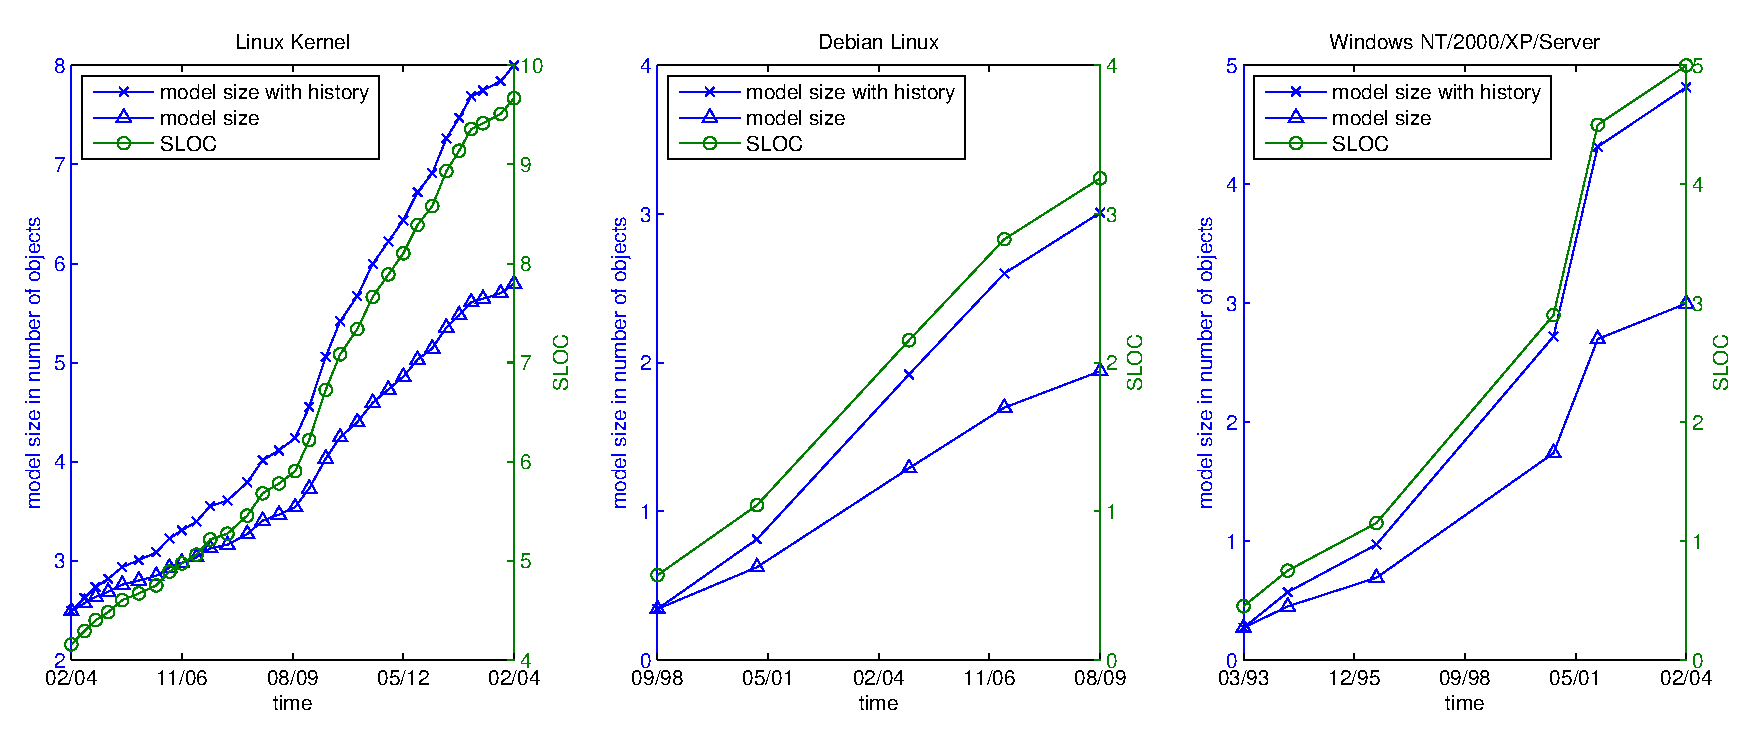
\includegraphics[width=\linewidth]{figures/software_model_sizes}
  \caption{SLOC and estimated number of objects for popular large software projects.}
  \label{fig:software_model_sizes}
\end{figure}


We also transferred all ratios from the Kernel to other OS software projects and publicly reported LOC counts. The results are presented in Fig.~\ref{fig:software_model_sizes}. As you can see, these large software models can have a size upto a magnitude of $10^9$ objects.

Furthermore, it is not clear whether further grow in software project size is exponential or linear. 
Some believe that software size follows Moore's Law. Others think that software is bound by increasing complexity and not by the limitations of underlying hardware.

\subsubsection*{Modeling Tasks}
There are two major use cases in today's software development: editing and analysing/transforming/compiling. The first is done based on diagrams (graphical editing) or compilation units (e.g. Java-files, textual editing). Diagram contents roughly corresponds to package contents. Both packages and compilation units are sub-trees within the whole containment tree of the software model. Analysing, transformation, and compiling is usually either done for the whole model or again on a per package or compilation unit basis. Within these aggregates, the use-case usually requires to traverse the model. An exception can be the analysis based on single queries. But due to performance issues, model analysis is usually performed by traversing the model and executing queries more like model transformations. Software models are only accessed by a view individuals at the same time.

%\subsubsection{What are software code models?}
%We use the term model to describe MDSD artifacts. Originally these artifacts were models on a high level of abstraction, but today programming code, can also be understood as models. For example IDEs such as eclipse JDT or eclipse CDT internally maintain programming code as ASTs (primitive models) in order to provide advanced IDE features such as outlines, error annotations, type and call hierarchies, and code completion. It is safe to assume that programming code contains far more information compared to high-level models. Since we are looking for extra large models, we will concentrate on software code models.
%
%Advances in language workbenches suggest to replace these IDEs with eclipse EMF based and generated tools. Advances in comparison and versioning of models will soon allow to replace per-line-text-file-based versioning systems (e.g. CSV, SVN, GIT) with model based (e.g. EMF-based) systems that version on a per mode-object- or even per-object-attribute basis.
%
%\subsubsection{How big is are existing software code models?}
%How large are these software code models? Traditionally code size is measured in \emph{lines of code} LOC (physical lines), SLOC (source LOC, like LOC but without empty lines, comments, duplicates; refer to Wheeler~\cite{wheeler}, and LLOC (logical LOC, like SLOC but normalized to one statement per line). These measures exist for many known software projects (and their history) and can be easily captured for open source projects. 
%
%In order to determine corresponding model sizes, we need to know how much model objects each LOC represents. To estimate this, we used the eclipse CDT parser as tool and the linux kernel as sample. The CDT parser is specialized to parse C/C++ code in its un-preprocessed form. Thus, the resulting ASTs are not bloated with information injected (with lots of duplicates) during pre-processing. Of course ASTs are not software models as they are understood in the OMG/EMF world, but we can assume that proper C/C++ models will contain one object for each AST node. \markus{This needs a reference}. Parsing the current kernel version, counting its AST nodes, and comparing this number to the kernel's SLOC number gives us a good estimate for objects per SLOC (at least for the kernel code, probably for all C code, and maybe it is also a good estimate for other similar programming languages, e.g. C\#, Java). We will use this estimate to extrapolate the model size of other kernel versions and other software projects. 
%
%Eventually, we want to store software models and its versions. Of course, we only want to store the differences between versions. A software projects model size is determined by the size of the differences that produced the current software model. To determine this size, we need to know how much LOCs were added, removed, and modified in a software project. To estimate this, we use the versioning system GIT as tool and the linux kernel GIT repository as sample. With gitstats we can determine the number of added, removed, and changed lines throughout the repository history. With these numbers, the estimated objects per SLOC and the recorded SLOCs for different kernel versions we can estimate the model size of a kernel software code model repository. We can also assume that other software projects have a similar proportion of added, removed, and modified lines, and transfer these estimates to other software projects. 
%
%\begin{figure}
%  \centering
%  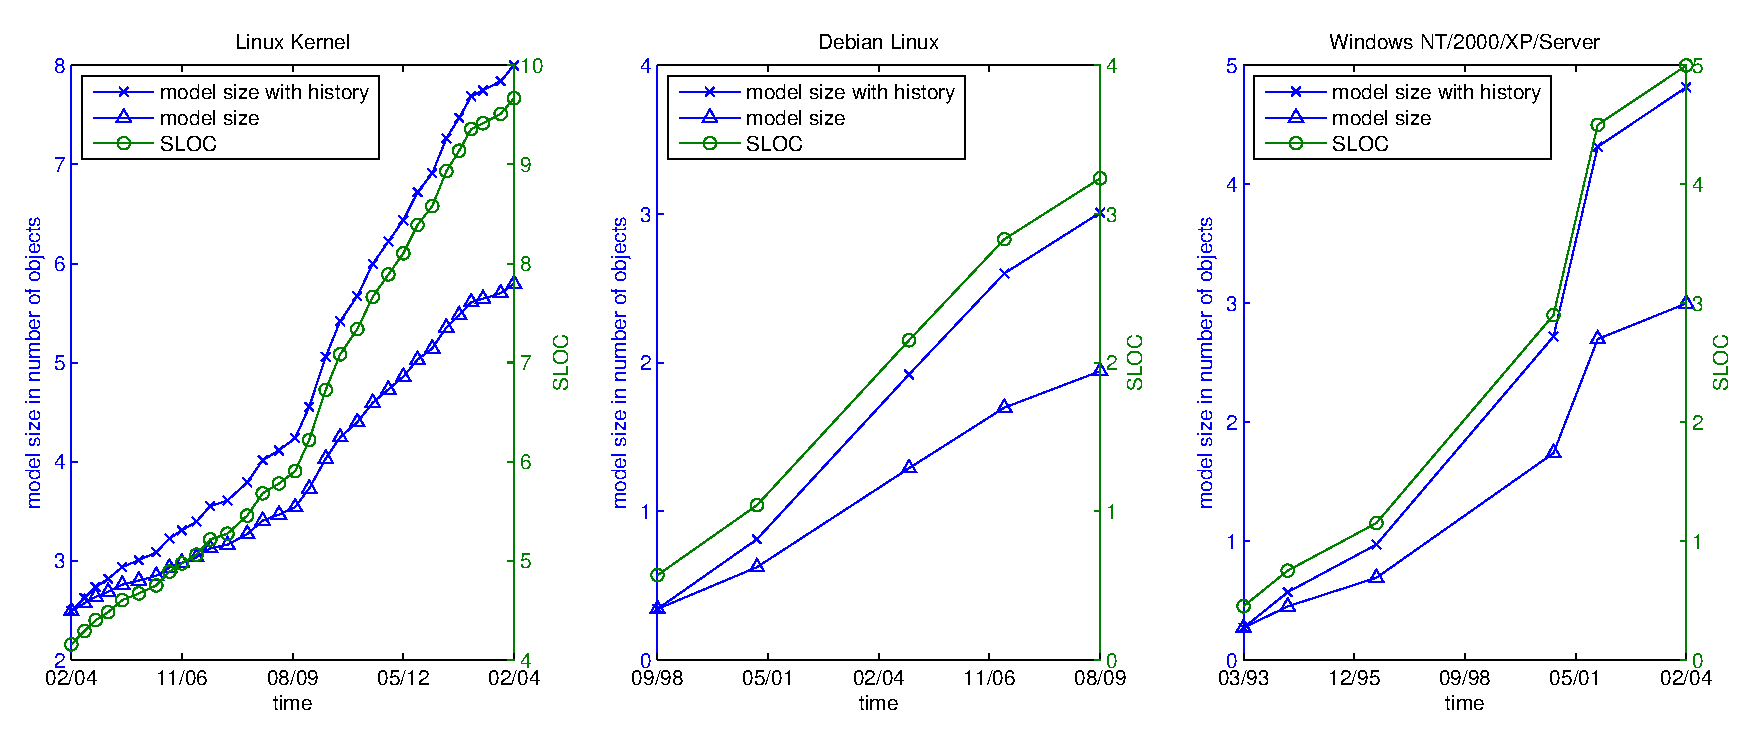
\includegraphics[width=\linewidth]{figures/software_model_sizes}
%  \caption{SLOC and estimated number of objects for popular large software projects.}
%  \label{fig:software_model_sizes}
%\end{figure}
%
%Fig.~\ref{fig:software_model_sizes} shows the LOC numbers and estimated object numbers in corresponding software code models. The charts present different software projects and how size developed over time. \markus{kernel, linux(debian)?, windows - numbers based on kernel git alone, SLOC numbers and transferred kernel estimates.}
%
%\subsubsection{How big are software code models in the future?}
%
%Some believe that the average size software (and software code models for that matter) grows faster than linear following Moore's Law. Maciej Soltysiak for example has analysed the grows of the linux kernel code base and observed exponential growth. A counter argument is that software not only bound by hardware limitations (i.e. Moore's Law) but increasingly by software complexity and therefore will not grow exponentially. Never the less, it is safe to assume that software code models will be larger in the future.

\subsection{Heterogenous Sensor Data}

Sensor data usually comprises of time series of measured physical values in the environment of a sensor; but sensor data can also contain patterns of values (e.g. video images). Sensor data is collected in sensor networks, that combine distributes sensors with an communication infrastructure. Sensor data can be heterogeneous: a sensor network can use different types of sensors that measure a multitude of parameters. \markus{cites, cites, cites}. 

We build the \emph{Humboldt Wireless Lab} are 120 node wireless sensor network. Nodes are equipped with 3 axis accelerometer, but more essentially for our research also creates data from monitoring all running software components (mostly networking protocols), and other system parameters (CPU, memory, or radio activity, etc.). We represent analyse this data as EMF ecore based models (e.g.~\cite{SMTLpaper}).

\subsubsection*{Model Size}
HWL network protocol and system software components provide 372 distinct data sets (containing data such as WLAN radio data, network statistics, CPU load levels, etc.) Each data set is represented in an XML fragment of variable size. Per second each node in the network produces XML entities that translate into an average of 1120 EMF objects. A common experiment with HWL involves 50 nodes and measures of a period of 24h. Such an experiment produces a model of $5*10^9$ objects. 

In general, sensor networks are currently only limited by the limitations of the technical infrastructure that supports them. Ambiguous computing and Smart Citys \markus{cites} suggest sensor data models of arbitrary sizes. 

\subsubsection*{Modeling Tasks}
There are two major use-cases recording sensor data and analysing sensor data. Recording sensor data means to store it faster then it is produced. If possible in a manner that supports later analysis. Sensor data is rarely manipulated. Analysis means to access individual data sets (sub-trees) and to traverse these data sets (mostly time series). Analysis is usually done by only a single (or a few) individuals at the same time. 


\subsection{Geospatial Models}

3D city models are a good example for structured geo-spatial information. The CityGML standard, provides a set of xml-schemas (building upon other standards, e.g. GML) that function as a meta-model. CityGML, compared to other quasi standards (e.g. google KML) does not solely concentrate on the 3D measures, but allows to extend the covered information by more semantic attributes (e.g. materials, age, inhabitants, existing infrastructure, etc.). Geo spatial models usually come with different levels of details (LOD); CityGML distinguishes 5 LODs, 0-4) \markus{cite}. 

\subsubsection{Model Size}
Like many cities, Berlin is currently establishing such a model. The current model of Berlin comprises all of Berlin, but mostly on a low-medium level of detail (LOD 1-2). To get an approximation of the model's size, we counted the XML entities. The current Berlin model, contains roughly $128*10^6$ objects. 

Based on data published in~\cite{CityGMLBerlinDB} a LOD 1 building comprised of 12.5 objects, a LOD 2 building of 40 objects, a LOD 3 building of 350 objects. A LOD 3-4 building of Berlin would therefore consist of $1*10^9$ objects. Berlin inhabits 3.5 million people. About 50\% of the worlds $7*10^9$ people live in cities. This gives a whole LOD3-4 approximation of $10^{12}$ objects for a \emph{world 3D city model}.

\subsubsection{Modeling Tasks}
Geo-spatial models are accessed by many people at the same time. Compared to model manipulation, model access (partial load) is far more common and its efficient execution is paramount. If accessed, users usually load a containment hierarchies (sub-tree) corresponding to a given set of coordinates or address (geographic location). Queries for distinct feature characteristics within a specific geographic location (i.e. with-in such containment hierarchies) is also common. 



